\section{ON STATION}

\subsection{Combat Air Patrol}

A Combat Air Patrol (CAP) is a patrol provided over an objective area, a force
to be protected, or defense area, for the purpose of intercepting and
destroying hostile aircraft before they reach their expected target(s).

\sidebyside{0.625}{

  CAP patterns are often racetracks, to be flown at optimum endurance speed
  (Tactical Brevity Codeword: \textbf{SAUNTER}) at an altitudes high enough to
  secure fuel conservation whilst managing sensor deployment effectively, i.e.
  look-down.

  The pattern is defined by an \textbf{Anchor Point}, marking the entry point
  of the first turn along with a leg distance or duration.

  When determining Anchor point parameters, consider the compromise between
  radar scan time in the threat direction vs. how close from the Anchor
  Point you wish to to stay which impacts your reaction time, airspace
  structure, and geographical factors.

  High altitude patrols come with an increased chance of detection and
  diminishes the element of surprise and represents a tactical consideration
  to be made. Low CAPs are possible, and the mission commander will define the
  legs, direction and altitude of the CAP anchor, with 20,000 feet being a
  reasonable compromise.

}{%
  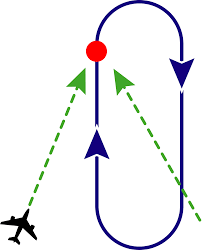
\includegraphics[width=\textwidth,align=t]{aar/cap}%
}

\subsection{Scan responsibilities and splitting}

The sensor mate contract covered in \fullref{sec:contracts-sort-scan} should
be in effect following our FENCE check but remains crucial for an effective
CAP. This ensures all altitude blocks are covered with the razors edge crossed
by 5,000 feet and the Wingman scanning near and low blocks, the lead covering
far and high.

\subsection{CAP Planning Considerations}

Whist normal doctrine requires a flight to maintain integrity at all times,
DataLink and Yardstick are technologies that enhance the distance a flight
may split without losing operational integrity.

As such splitting a flight to ensure that hot legs (those pointing in the
threat direction) have near-permanent coverage may improve threat detection
whilst costing increased radar management (full altitude coverage per
aircraft). Aditionally, it provides the ability to get into a number of
tactical formations prior to a BVR engagement.

When splitting the flight (or elements), the length of the track legs
should not exceed the maximum trail length in a split trail engagement, or the
distance beyond which mutual support extends. This can be anywhere from 5 NM
for Sidewinder to 20 NM for Phoenix.